
\section{Impossibility of Exact Shifting within Positive Fields}
\label{sec:shifting_lower_bound}

In this section, we present an example  showing that, within a positive field,
we cannot shift positive requests down, obtaining $\alpha$ requests in every
node, like we did in the case of negative requests
(cf.~\lref[Corollary]{cor:crucial_lemma_neg}). In our construction, the tree 
$T$~consists of root $r$ and
two distinct subtrees $T_1$ and $T_2$, each of size $s$ and containing $\ell$
leaves.

\balance

Suppose that, at the beginning, \ALG has the entire tree~$T$ in its cache and
the following ordered events happen (cf.~\lref[Figure]{fig:trbl_exmpl}).
\begin{enumerate}
\item \ALG evicts $T_1 \cup \{ r \}$ from the cache.
\item $(s+1) \cdot \alpha - \ell$ requests appear one by one at $r$. The number of
  requests is too small to trigger a fetch of any subtree of $T_1 \cup \{ r \}$.
\item \ALG evicts $T_2$ from the cache.
\item $s \cdot \alpha$ requests appear one by one at the root of $T_1$. This
  time, the number of requests is too small to trigger a fetch of any
  subtree of $T$.
\item $\ell$ requests appear one by one at $r$. After the last one appears,
  {\ALG} fetches the entire $T$ to the cache.
\end{enumerate}
The evictions happen because of some feasible sequence of negative requests that
is irrelevant from our perspective.

\begin{figure}[t]
  \centering
  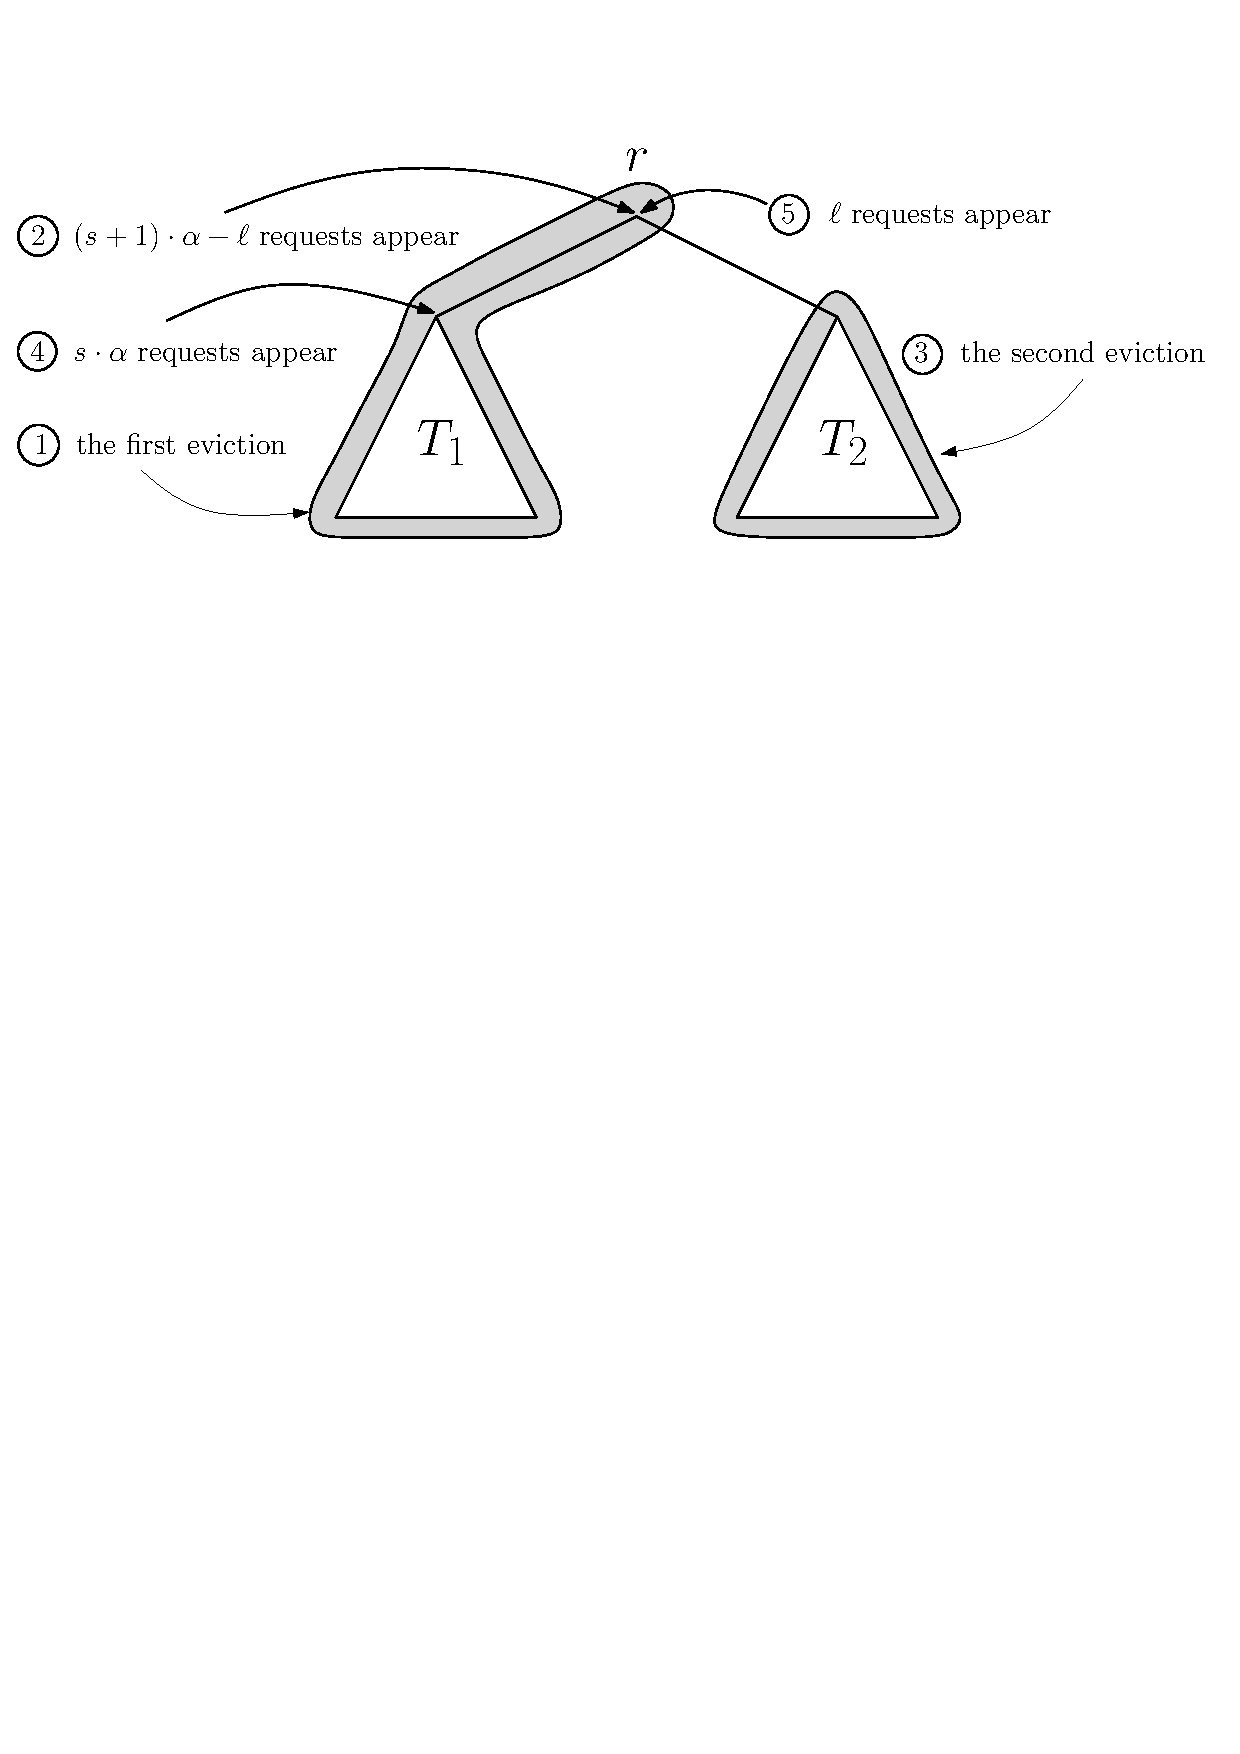
\includegraphics[width=0.9\columnwidth,keepaspectratio]{images/example}
  \caption{A troublesome example of a positive field. Numbers in circles describe 
  the chronology of the events.}
  \label{fig:trbl_exmpl}
\end{figure}


Now, observe that when requests appear at the root in the second stage of our
construction, $T_2$ is still in the cache (i.e., does not belong to the field
yet). Thus, all the requests, except for the last $\ell$ ones can be shifted
down only to nodes from $T_1$. Hence, for large $\alpha$ and~$s$, shifting can
deliver $\Omega(\alpha)$ requests only to half of the nodes.


